Wie eben diskutiert, koppelt die starke Wechselwirkung an Teilchen, die Farbladung tragen.
Die Farbladung hat hierbei drei m\"ogliche Zust\"ande: rot, blau und gr\"un.
Dabei spielt der Zustand der Farbladung f\"ur die St\"arke der starken Wechselwirkung keine Rolle.
Zus\"atzlich zu den drei Zust\"anden der Farbladung gibt es auch drei Zust\"ande der Antifarbladung, antirot, antiblau und antigr\"un.
%Die Farbladung enth\"alt jedoch keine Information \"uber die optische Farbe der Teilchen.
\newline
Die Kombination der drei (Anti-)Farbladungen, oder die Kombination von Farbladung mit entsprechender Antifarbladung ergibt, angelehnt an die Farblehre, wei{\ss}.
Teilchen mit einer solchen Kombination der Farbladung ergeben entsprechen nach au{\ss}en hin farbneutralen Teilchen, auch wenn sie aus farbgeladenen Teilchen aufgebaut sind.
\newline
Quarks, Antiquarks und Gluonen tragen Farbladung, wodurch sie an der starken Wechselwirkung teilnehmen.
%% Satz zu lange
Unter anderem bindet die starke Wechselwirkung Quarks und Antiquarks zu sogenannten Hadronen, die wiederum in sogenannte Baryonen, aufgebaut aus drei Quarks, und sogenannte Mesonen, aufgebaut aus einem Quark-Antiquark-Paar und entsprechende Antiteilchen, unterteilt werden.
%%
%In der Natur kommen nur farbneutrale Teilchen frei vor, entsprechend gibt es (Anti-)Quarks nur in Zusammenschl\"ussen zu anderen Teilchen. 
%Dieses Ph\"anomen wird als \textit{Confinement} bezeichnet.
%Um das \textit{Confinement} besser verstehen zu k\"onnen wird im Folgenden das Potential der starken Wechselwirkung betrachtet.
\newline
Die Wechselwirkung zur Bindung eines Quark-Antiquark-Paars folgt dabei einem Potential $V(r)$ \cite{script:kt1}:
\begin{align} \label{eq:Potential}
V(r) = -\frac{4}{3}\frac{\alpha_\text{s}}{r} + kr 
\end{align}
%%%%%%%%%%%%%%%%%%%%%%%%%%%%%%%%%%%%%%%%%%%%%%%%%%%%
% erst Potential ohne alpha_s(r)
% dann ueber running alpha_s(r)
%%%%%%%%%%%%%%%%%%%%%%%%%%%%%%%%%%%%%%%%%%%%%%%%%%%%
Der absto{\ss}ende Teil $-\frac{4}{3}\frac{\alpha_\text{s}}{r}$ verh\"alt sich proportional zur sogenannten Kopplungskonstanten der starken Wechselwirkung $\alpha_{\text{s}}$ und antiproportional zum Abstand $r$ zwischen Quark und Antiquark.
Anders als die Bezeichnung vermuten l\"asst ist die Kopplungskonstante der starken Wechselwirkung nicht konstant, sondern abh\"angig von $r$.
Je kleiner $r$ wird, umso kleiner wird $\alpha_{\rm{s}}$.
Aufgrund dieses Verhaltens von $\alpha_{\rm{s}}$ bez\"uglich $r$ nennt man $\alpha_\text{s}$ auch laufende Kopplungskonstante.
\newline
Der anziehende Teil des Potentials $+kr$ weist eine lineare Abh\"angigkeit von $r$ auf.
Der Vorfaktor $k$ wird als Stringspannung bezeichnet und liegt in der Gr\"o{\ss}enordnung von etwa 1 GeV/fm.
F\"ur gro{\ss}e Abst\"ande dominiert der anziehende Teil.
Das Feld der starken Wechselwirkung zwischen den beiden Teilchen wird immer st\"arker und wird deshalb als \textit{String} bezeichnet.
%%%%%%%%%%%%%%%%%%%%%%%%%%%%%%%%%%%%%%%%%%%%%
Um den Abstand zwischen sich zu vergr\"o{\ss}ern, m\"ussen die zwei Teilchen immer mehr Energie besitzen, die insgesamt gleich der Energie des \textit{String} entspricht.
Ab einem bestimmten Abstand reicht die Energie in dem \textit{String} aus, um ein weiteres Quark-Antiquark-Paar zu erzeugen.
In dem String bildet sich ein neues Quark-Antiquark-Paar, das sich mit dem urspr\"ungliche Quark-Antiquark-Paar zu zwei Quark-Antiquark-Paaren kombiniert.
Es liegen dann zwei Quark-Antiquark-Paare vor, die jeweils aus einem urspr\"unglichen Teilchen und einem neu entstandenen Teilchen bestehen.
Deshalb k\"onnen Quarks nur in gebundenen Zust\"anden gemessen werden.
Dieses Ph\"anomen wird als \textit{Confinement} bezeichnet.
Aus dem \textit{Confinement} folgt, dass in der Natur nur farbneutrale Teilchen frei vorkommen, sprich (Anti-)Quarks bilden immer andere Teilchen.%
\newline
F\"ur kleine $r$ geht die St\"arke des Potentials gegen 0, da $\alpha_\text{s}$ schneller als $r$ kleiner wird.
Farbgeladene Teilchen sp\"uren in diesem Fall nur eine kleine Wechselwirkung.
Halten sich viele (Anti)Quarks und Gluonen auf kleinem Raum auf, so befindet sich ein Teilchen immer nah an einem anderen Teilchen.
Dadurch k\"onnen sich die Teilchen innerhalb eines solchen Zustands quasi frei bewegen.
Den Zustand, wenn sich farbgeladene Teilchen frei bewegen k\"onnen, nennt man asymptotische Freiheit.
\newline
Eine theoretische Beschreibung eines solchen Zustands ist das sogenannte Quark-Gluon-Plasma (QGP).
Das QGP entspricht einem Medium mit hoher Dichte von (Anti)Quarks und Gluonen und beziehungsweise oder hoher Temperatur.
\begin{figure}[tp]
\centering
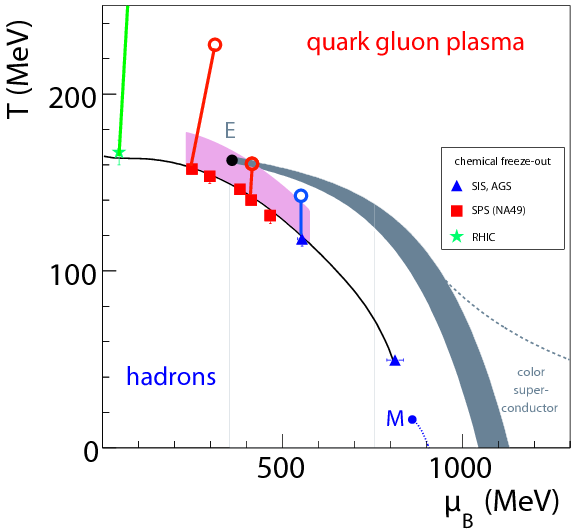
\includegraphics[width=.6\linewidth]{Phasediagram_Points-2008-neu.png}
\caption{Phasendiagramm stark wechselwirkender Materie in Abh\"angigkeit der netto Baryonendichte $\mu_{\text{B}}$ und der Temperatur $T$.
\cite{PAPER:Phasediagaram}}
\label{fig:QGPPhase}
\end{figure}
\newline
Ein solcher hei{\ss}er und dichter Zustand kann kurz nach der Kollision von zwei hochenergetischen Atomkernen entstehen.
In der \"Uberlappregion der beiden Atomkerne bildet sich ein QGP aus, das expandiert und abk\"uhlt.
Durch das Expandieren und Abk\"uhlen \"andert sich der Zustand des Mediums und die farbgeladenen Teilchen schlie{\ss}en sich in der sogenannten Hadronisierung wieder zu Hadronen zusammen.
Bei dem beschriebene \"Ubergang des QGP in hadronische Materie handelt es sich um einen Phasen\"ubergang stark wechselwirkender Materie.
%Diese Hadronen k\"onnen zerfallen, insofern sie keine stabilen Teilchen sind.
%Es kann auch zu ganzen Zerfallsketten kommen, bis die Endteilchen nicht mehr zerfallen.
%Je nach dem, wie schnell Teilchen zerfallen, k\"onnen entweder diese oder ihre Zerfallsprodukte gemessen werden und geben indirekt Aufschluss auf Eigenschaften des hei{\ss}en und dichten Mediums.
\newline
F\"ur die Erforschung des QGP spielt das Phasendiagramm stark wechselwirkender Materie eine wichtige Rolle.
Abbildung \ref{fig:QGPPhase} skizziert das Phasendiagramm stark wechselwirkender Materie in Abh\"angigkeit von der Baryonendichte $\mu_{\text{B}}$ und der Temperatur $T$.
Bei geringem $\mu_{\text{B}}$ und niedrigem $T$, wie etwa Raumtemperatur, sind alle Quarks und Gluonen in Hadronen gebunden.
Erh\"oht man $T$ oder beide Gr\"o{\ss}en stark, wird ein \"Ubergang in das QGP erwartet, in dem sich die Quarks und Gluonen quasi frei bewegen k\"onnen.
Au{\ss}erdem muss die Energiedichte gro{\ss} genug sein, um ein QGP erzeugen zu k\"onnen, weshalb davon ausgegangen wird, dass sich dieses bei Kern-Kern-Kollisionen im Labor ausbilden kann.
Es wird davon ausgegangen, dass im fr\"uhen Universum kurz nach dem Urknall die gesamte Materie als QGP vorlag.
\newline
Der experimentelle Aufbau f\"ur Kollisionsexperimente wird in Abschnitt \ref{s2} n\"aher beschrieben.
In dieser Arbeit werden allerdings Proton-Proton-Kollisionen betrachtet, die unter anderem als Referenz f\"ur Kern-Kern-Kollisionen benutzt werden k\"onnen. 
%Im n\"achsten Abschnitt werden zun\"achst die Grundlagen zur Analyse neutraler Pionen erkl\"art.


%Der Aufbau eines Kollisionsexperiments wird in Abschnitt \ref{s3} n\"aher erl\"autert.


%F\"ur gro{\ss}e $r$ wird der anziehende Teil also immer stärker.
%Will man also zwei farbgeladene Teilchen wie etwa ein Quark-Antiquark-Paar von einander trennen, so m\"usste man immer mehr Energie aufwenden, je weiter man die Teilchen von einander entfernt.
%Diese Erzeugung eines neue Quark-Antiquark-Paares findet immer statt sobald sie m\"oglich ist.
%Deshalb sind Quarks und Gluonen nicht direkt einzeln messbar, was die Untersuchung von Quarks, Gluonen und der starken Wechselwirkung erschwert.
%Um zu erkl\"aren, wie die starke Wechselwirkung, Quarks und Gluonen trotzdem untersuchen werden k\"onnen muss man sich $\alpha_\text{s}$ genauer anschauen. 
%\begin{figure}[thp]
%\centering
%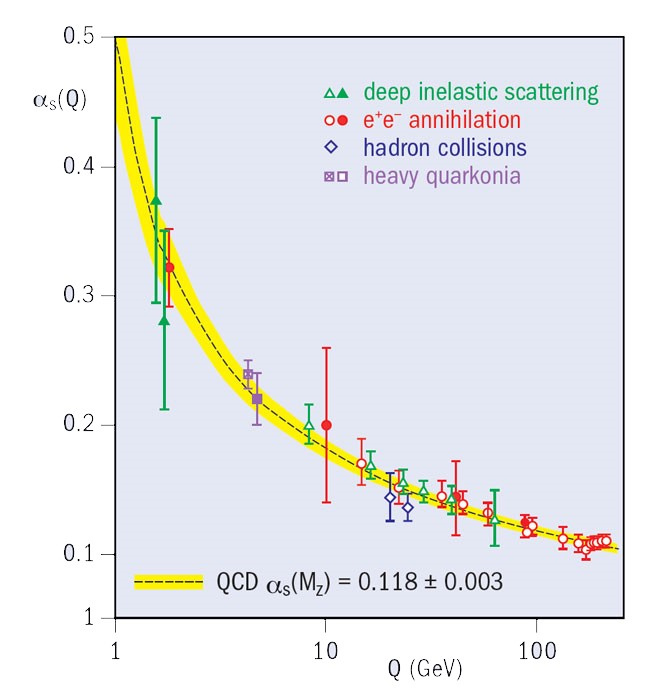
\includegraphics[width=.5\linewidth]{alpha_s.jpg}
%\caption{Die Kopplungskonstante der starken Wechselwirkung $\alpha_\text{s}$ in Abh\"angigkeit des Impulsübertrags $Q$. Eingezeichnet befinden sich Messpunkte unterschiedlicher Experimente, sowie in gelb eine theoretische Rechnung.
%\cite{article:1}}
%\label{fig:alpha_2}
%\end{figure}
%Stattdessen h\"angt $\alpha_\text{s}$ vom sogenannten Impulsübertrag $Q$ zwischen zwei Teilchen ab.
%Abbildung \ref{fig:alpha_2} zeigt den Verlauf von $\alpha_\text{s}$ in Abh\"ahngigkeit von $Q$.
%Der Impulsübertrag $Q$ h\"angt dabei selbst \"uber die De-Broglie-Wellenl\"ange mit dem Abstand $r$ zusammen.
%Es gilt $Q = \frac{h}{\lambda}$, wobei $\lambda$ die r\"aumliche Aufl\"osung beschreibt.
%F\"ur eine genau Aufl\"osung, also f\"ur  sehr kleine $r$ muss entsprechend $Q$ gro{\ss} sein.
%$\alpha_\text{s}$ h\"angt also antiproportional von $r$ ab.